\chapter{Cadre général du projet}
\renewcommand{\thesection}{\arabic{section}}
\vspace{-1cm}
\begin{justify}
    \section*{\texorpdfstring{Introduction}{Introduction}}
    \addcontentsline{toc}{chapter}{\textbf{Introduction}}
    Ce premier chapitre présente le contexte général du projet et l’organisme d’accueil, en analysant et en critiquant les solutions existantes ainsi que l’état actuel de la première version l’application, tout en mettant en évidence leurs limites afin de justifier la nécessité d’une nouvelle approche. Il expose également la solution proposée ainsi que la méthodologie adoptée pour sa mise en œuvre.
    \section{\texorpdfstring{Contexte général du projet}{Contexte général du projet}}
    Dans le cadre de l'obtention du diplôme national d'ingénieur en génie informatique, spécialité \ac{NTS}, à l'\ac{ENSIT}, une opportunité a été offerte pour réaliser un projet de fin d'études au sein de la société ADDINN Tunisie, au sein de l'équipe \ac{QA}, pour une durée de quatre mois, durant l'année universitaire 2024/2025.
    \section{Présentation de l’organisme d’accueil}
    Dans cette section, nous présentons l’organisme d’accueil en abordant son histoire, ses valeurs, ainsi que ses partenariats qui contribuent à son succès et à son développement.
\subsection{\texorpdfstring{Aperçu général d'Addinn}{Aperçu général d'Addinn}}
    \begin{minipage}{.6\textwidth}
        \justifying
        Addinn est un cabinet de conseil en transformation digitale spécialisé dans l’accompagnement des entreprises pour définir leur stratégie et mettre en œuvre leurs projets technologiques grâce à un écosystème innovant et complémentaire permet de relever les défis numérique avec succès\cite{Addinn}.\\
    \end{minipage}
    \begin{minipage}{.4\textwidth}
        \vspace{-2.1cm}
        \begin{figure}[H]
            \centering
            
\includegraphics[width=\linewidth]{pages/page-de-garde/img/logo.png}
            \caption{\centering Logo d'\acs{ADDINN}\protect{\cite{Addinn}}}
            \label{fig:logo-ADDINN}
        \end{figure}
    \end{minipage}
\vspace{-0.8cm}
\subsection{Fondements de la Société\cite{apropos}}
    \acs{ADDINN} a pour mission de créer de la valeur à chaque étape de la réflexion à la mise en œuvre et au déploiement des projets \acs{IT}. Son engagement en faveur de l’innovation se reflète dans sa devise "\textbf{ADD} VALUE BY \textbf{INN}OVATION", illustrant sa volonté d’apporter une réelle valeur ajoutée à ses clients. Grâce à son approche novatrice et son expertise, l'entreprise aide à relever les défis avec agilité et efficacité, garantissant ainsi une transformation réussie et durable.\\
    Le tableau~\ref{tab:objectifs} présente les objectifs et les valeurs qui orientent l’approche d’ADDINN:
    \begin{table}[H]
        \centering
        \caption{Synthèse des objectifs stratégiques et des valeurs portées par ADDINN}
        \renewcommand{\arraystretch}{1.5}
        \begin{tabular}{|c|c|}
            \hline
          \textbf{ Objectifs d’ADDINN }  & \textbf{Valeurs d’ADDINN}\\ \hline
            \begin{minipage}{.48\textwidth}
                \vspace{0.15cm}
                 \begin{justify}
                    \begin{itemize}[label=$\bullet$,left=-0.1cm]
                        \item Optimiser les flux de travail afin de les rendre plus rapides et simples.
                        \item Développer des systèmes et des solutions plus efficaces.
                        \item Améliorer l'expérience de clients et accroître l'avantage concurrentiel de l'entité.
                    \end{itemize}
                \end{justify}
                \vspace{0.15cm}
            \end{minipage}
              & 
            \begin{minipage}{.48\textwidth}
                \vspace{0.15cm}
                 \begin{justify}
                    \begin{itemize}[label=$\bullet$,left=-0.1cm]
                        \item \textbf{Innovation}: Pousser plus loin les idées grâce à la recherche et au développement.
                        \item \textbf{Agilité}: Reposer sur la flexibilité et la collaboration comme principes fondamentaux.
                        \item \textbf{Excellence}: Viser la qualité à travers une approche structurée et optimisée.
                    \end{itemize}
                \end{justify}
                \vspace{0.15cm}
            \end{minipage} \\\hline
        \end{tabular}
        \label{tab:objectifs}
    \end{table}
    \vspace{-0.6cm}
\subsection{Fiche de présentation d'ADDINN}
        Le table ~\ref{tab:infoADD} fournit un aperçu détaillé de l'organisme d'accueil.
        \begin{table}[H]
            \caption{\centering Fiche de présentation de la société d'ADDINN \cite{Addinn}\cite{apropos}} 
            \centering
            \renewcommand{\arraystretch}{1.5}
            \begin{tabular}{|p{2.3cm}|p{14cm}|}
                \hline
                    \textbf{Nom} & \textbf{ADDINN}\\
                \hline
                    \textbf{Type} & Société de conseil en transformation digitale\\
                \hline
                    \textbf{Adresses} & 
                        \begin{minipage}{14cm}
                            \begin{justify}
                                \vspace{0.15cm} 
                                \begin{itemize}[left=-0.1cm,label=$\bullet$]
                                    \item \textbf{ADDINN Groupe (France):} 121 Avenue Champs-Elysées Paris 75008.
                                    \item \textbf{ADDINN Tunis:} Immeuble Etraton, Rue Khadija Ben Arfa, Centre Urbain Nord 1082.
                                    \item \textbf{ADDINN Sousse:} Rue Hedi Nouira Akouda Sousse 4022.
                                    \item \textbf{ADDINN Tozeur:} Immeuble Akouri, 2ème étage, rue 2 Mars, Tozeur.
                                    \item \textbf{ADDINN Africa (Congo Brazzaville):} N°3 Allée des Manguiers Beach Centre-ville – Brazzaville.
                                \end{itemize}    
                                \vspace{0.15cm}        
                            \end{justify}
                        \end{minipage}\\
                \hline
                    \textbf{Chiffres Clés} & 
                        \begin{minipage}{14cm}
                            \vspace{0.15cm} 
                            \begin{itemize}[left=-0.1cm,label=$\bullet$]
                                \item Plus de 11 ans d’expérience en consulting IT.  
                                \item Plus de 100 consultants et ingénieurs qualifiés.  
                                \item 90\% des projets gérés en Agile/Scrum.  
                                \item Plus de 40 experts certifiés.  
                            \end{itemize}
                        \end{minipage}\\
                \hline
                    \textbf{Domaines d'expertise} & Conseil en stratégie, conseil en transformation digitale, développement IT et solutions numériques. \\
                \hline 
                    \textbf{Email} & 
                        contact@addinn.com et sales@addinn.com \\
                \hline
                    \textbf{Site web} & \url{https://addinn-group.com/}\\
                \hline
            \end{tabular}
            \label{tab:infoADD}
        \end{table} 
    \vspace{-0.5cm}
    \subsection{Histoire de croissance d’ADDINN et présence internationale\cite{apropos}}
        L’histoire d’ADDINN débute en 2012, avec la rencontre de deux amis ambitieux souhaitant prendre part à la révolution digitale. Plus d’une décennie d’efforts, d’innovations technologiques et de stratégie d’expansion a permis à l’entreprise de franchir ses frontières d’origine.
        \begin{minipage}{.55\textwidth}
            \begin{justify}
                Aujourd’hui, ADDINN Group s’impose comme un acteur clé du marché euro-méditerranéen et africain. Avec son siège social à Paris, le groupe a étendu ses activités en créant 3 filiales en Tunisie, en Mauritanie et au Congo-Brazzaville , comme le montre la figure~\ref{fig:presence_addinn}.
                
                Grâce à des partenariats solides, ADDINN maintient des relations privilégiées avec ses clients au Gabon, en République Démocratique du Congo et en Belgique, consolidant ainsi son expansion à l'international.  
                
                Le tableau~\ref{tab:etapes_addinn} résume les étapes clés de cette croissance.
            \end{justify}
        \end{minipage}
        \hspace{0.1cm}
        \begin{minipage}{.45\textwidth}
            \vspace{-1cm}
            \begin{figure}[H]
                \centering
                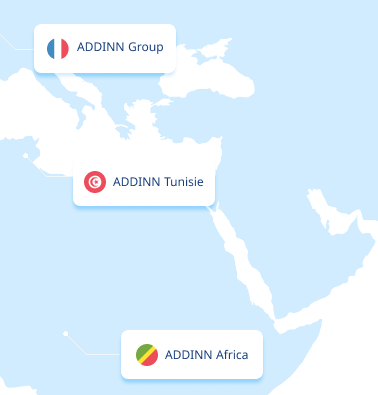
\includegraphics[width=\linewidth]{chapitres/ch1/img/map.PNG}
                \caption{\centering Présence internationale d'ADDINN\cite{apropos}}
                \label{fig:presence_addinn}
            \end{figure}
        \end{minipage}
        \begin{table}[H]
            \centering
            \caption{Étapes Clés d'Évolution d’ADDINN\cite{apropos}}
            \renewcommand{\arraystretch}{1.5}
            \begin{tabular}{|l|p{15cm}|}
                \hline
                \textbf{Année} & \textbf{Événement} \\
                \hline
                \textbf{2015} & Fondation d’ADDINN Group en France, spécialisé dans le conseil en IT. \\
                \hline
                \textbf{2018} & Création de la Digital \& Software Factory, dédiée au développement de solutions numériques sur mesure. \\
                \hline
                \textbf{2022} & Filialisation du groupe avec la création d’ADS Foundry, BeeWay Advisory et Qualifactory, ouvrant une nouvelle phase de développement et de croissance.  \\
                \hline
            \end{tabular}
            \label{tab:etapes_addinn}
        \end{table}
    \vspace{-0.6cm}
\subsection{Secteurs d'expertise et partenaires stratégiques} 
    L'expertise d'ADDINN couvre divers secteurs tels que l'assurance, la banque, le secteur public et le transport, offrant des solutions sur mesure. De plus, l'entreprise collabore avec plusieurs partenaires pour renforcer son offre et sa compétitivité, comme l'illustre la figure \ref{fig:Partenaires}.
    \vspace{-0.3cm}
    \begin{figure}[H]
        \centering
        \renewcommand{\thesubfigure}{}
        \subfloat{
\includegraphics[width=0.16\textwidth]{chapitres/ch1/img/partenaires/a1.png}}
        \subfloat{
\includegraphics[width=0.155\textwidth]{chapitres/ch1/img/partenaires/a2.png}} 
        \subfloat{
\includegraphics[width=0.13\textwidth]{chapitres/ch1/img/partenaires/a9.png}}
        \subfloat{
\includegraphics[width=0.14\textwidth]{chapitres/ch1/img/partenaires/a10.png}}
        \subfloat{
\includegraphics[width=0.15\textwidth]{chapitres/ch1/img/partenaires/a5.png}}
        \subfloat{
\includegraphics[width=0.15\textwidth]{chapitres/ch1/img/partenaires/a11.png}}
        \subfloat{
\includegraphics[width=0.14\textwidth]{chapitres/ch1/img/partenaires/a3.jpg}} \\
        
        \subfloat{
\includegraphics[width=0.17\textwidth]{chapitres/ch1/img/partenaires/a4.png}}
        \subfloat{
\includegraphics[width=0.19\textwidth]{chapitres/ch1/img/partenaires/a12.png}}
        \subfloat{
\includegraphics[width=0.19\textwidth]{chapitres/ch1/img/partenaires/a7.png}}
        \subfloat{
\includegraphics[width=0.14\textwidth]{chapitres/ch1/img/partenaires/a19.png}} 
        \subfloat{
\includegraphics[width=0.15\textwidth]{chapitres/ch1/img/partenaires/a6.png}}
        \subfloat{
\includegraphics[width=0.19\textwidth]{chapitres/ch1/img/partenaires/a17.png}}\\
        
        \subfloat{
\includegraphics[width=0.17\textwidth]{chapitres/ch1/img/partenaires/a13.png}}
        \subfloat{
\includegraphics[width=0.22\textwidth]{chapitres/ch1/img/partenaires/a8.png}}
        \subfloat{
\includegraphics[width=0.17\textwidth]{chapitres/ch1/img/partenaires/a14.png}}
        \subfloat{
\includegraphics[width=0.17\textwidth]{chapitres/ch1/img/partenaires/a15.png}} 
        \subfloat{
\includegraphics[width=0.17\textwidth]{chapitres/ch1/img/partenaires/a16.png}}
        \subfloat{
\includegraphics[width=0.135\textwidth]{chapitres/ch1/img/partenaires/a18.png}}\\
        \caption{Partenaires stratégiques d'ADDINN \cite{Addinn}}
        \label{fig:Partenaires}
    \end{figure}    
    \vspace{-0.7cm}
    \section{Étude de l’existant}
        \vspace{-0.1cm}
L’étude de l’existant permet d’identifier les points forts et les limites de l’application actuelle, ainsi que d’analyser les solutions similaires, afin d’orienter le développement d’une nouvelle version mieux adaptée aux besoins des utilisateurs.
\subsection{État actuel de l'application existante}
    L’application \textbf{PENTRA} (Figure~\ref{fig:PENTRA-V1-1}) constitue une première version d’un outil automatisé de tests de pénétration, développée dans le cadre d’un projet de fin d’études réalisé l’année précédente au sein de la société \textbf{ADDINN}. Elle a permis de poser les bases sur lesquelles s’appuient les évolutions futures envisagées dans le cadre de notre projet actuel.    
    \begin{figure}[H]
        \centering
        
\includegraphics[width=\linewidth]{Annexe/PENTRA-V1/1.PNG}
        \caption{\centering Interface de la page d'accueil PENTRA}
        \label{fig:PENTRA-V1-1}
    \end{figure}
    \vspace{-0.3cm}
    \subsubsection{Analyse de la solution existante}  
        Il s’agit d’une solution de détection des vulnérabilités web, reposant principalement sur l’intégration de deux outils de scan réputés, largement reconnus dans le domaine de la cybersécurité :
        \begin{itemize}[label=$-$]
            \item  \textbf{OWASP ZAP (Zed Attack Proxy)}: Un scanner open source développé par l’OWASP pour identifier les failles de sécurité dans les applications web, telles que les injections SQL, les failles XSS, les problèmes d’authentification ou les erreurs de configuration. Il propose des analyses actives et passives, une interface graphique riche, ainsi qu’une API permettant son automatisation.\cite{zap}.
            \item \textbf{Wapiti}: un outil open source d’analyse de vulnérabilités web basé sur des tests d’injection, qui scanne les sites web à la recherche de failles comme les injections de commande, les XSS ou encore les inclusions de fichiers. Il se distingue par sa légèreté et son approche modulaire.\cite{wapiti}.  
        \end{itemize}
         Cette solution est développée avec Angular (version 15), FastAPI et PostgreSQL, et intègre les fonctionnalités clés suivantes:
        \begin{itemize}[label=$\bullet$, left=0.2cm]
             \item \textbf{Gestion de l’authentification\footnote{Voir annexe A: Figures \ref{fig:PENTRA-V1-2} et \ref{fig:PENTRA-V1-3}}:} Interfaces d'inscription et de connexion permettant aux utilisateurs de créer un compte et d'accéder à la plateforme via leurs identifiants.
            \item \textbf{Lancement du scan\footnote{Voir Annexe A: Figure \ref{fig:PENTRA-V1-4}}:} L’utilisateur saisit l’URL du site web à analyser dans le champ prévu. Les 2 outils de scan sont lancés et fonctionnent en mode multithread, ce qui permet de traiter plusieurs requêtes simultanément et d’accélérer le processus.
            \item \textbf{Tableau des résultats du scan par outil\footnote{Voir annexe A: Figures \ref{fig:PENTRA-V1-7}, \ref{fig:PENTRA-V1-8} et \ref{fig:PENTRA-V1-9}}:} Deux interfaces présentant les résultats des scans sous forme de tableaux, avec la possibilité de télécharger les rapports détaillés au format PDF, offrant ainsi une vue d'ensemble des vulnérabilités détectées.
            \item \textbf{Paramétrage de l’envoi des rapports\footnote{Voir annexe A: Figure \ref{fig:PENTRA-V1-10}}:} permet de configurer l’envoi automatique des rapports vers Slack, Jira et par e-mail.
            \item \textbf{Tableaux de bord\footnote{Voir annexe A: Figures \ref{fig:PENTRA-V1-5} et \ref{fig:PENTRA-V1-6}}:} Chaque outil dispose de sa propre interface, affichant les résultats des scans, leur progression, ainsi que des charts graphiques statiques.
            \item \textbf{Gestion des profils\footnote{Voir annexe A: Figures \ref{fig:PENTRA-V1-11}}:} Permet aux utilisateurs de modifier leurs informations personnelles.
            \item \textbf{Gestion des utilisateurs et des rapports de scan\footnote{Voir annexe A: Figures \ref{fig:PENTRA-V1-12} et \ref{fig:PENTRA-V1-13}}:} L’administrateur peut gérer les comptes utilisateurs ainsi que consulter, organiser et superviser les rapports des scans.
        \end{itemize}
    \subsubsection{Limites et critiques de la solution existante}
    L’application présente plusieurs lacunes affectant son ergonomie, ses performances et ses fonctionnalités. Ces limitations doivent être corrigées pour améliorer son efficacité globale.
        \begin{itemize}[label=\textcolor{red}{\ding{56}}]
            \item \textbf{Problèmes liés aux processus de scan et à la génération des rapports:}\\
            Les processus actuels de scan et de génération de rapports présentent plusieurs lacunes qui nuisent à la clarté des résultats, à l’ergonomie des interfaces et à l’efficacité globale de l’analyse. Parmi les problèmes relevés, on peut citer :
                \begin{itemize}[label=$\bullet$, left=-0.05cm]
                    \item \textbf{Surcharge d’informations:} Les tableaux des résultats des scans et les rapports générés sont excessivement longs et contiennent souvent des informations inutiles.
                   \item \textbf{Affichage de résultats non optimisés et non pertinents :} La présence de vulnérabilités avec un compteur égal à zéro, ainsi que de champs excessivement détaillés ou peu utiles, nuit à la lisibilité et complique l’analyse des résultats. Ce manque d’optimisation rend l’interprétation des rapports plus difficile et chronophage.
                    \item \textbf{Incohérence dans la structure des tableaux:} Les colonnes varient entre les outils, compliquant la comparaison des résultats. De plus, l'absence de filtres ou d'options de recherche pour trier les données rend leur exploitation moins efficace.
                    \item \textbf{Problèmes de progression des scans:} Les outils affichent la progression différemment: ZAP utilise une barre de progression, tandis que Wapiti le fait sous forme textuelle indiquant les modèles scannés, ce qui crée une incohérence.
                    \item \textbf{Navigation peu intuitive entre les interfaces des résultats:} La navigation entre les interfaces est confuse, ce qui complique la lecture et l’interprétation des résultats, notamment sur les tableaux de bord de Wapiti et ZAP ainsi que sur les deux tableaux de résultats, rendant l’analyse des vulnérabilités plus difficile.
                    \item \textbf{Mauvaise gestion des scans simultanés:} Le système actuel ne gère pas correctement les lancements parallèles ou successifs de plusieurs scans par le même utilisateur ou par plusieurs utilisateurs. Cela provoque une surcharge du backend, des conflits d’accès aux ressources, voire un blocage partiel de l’application. De plus, certains outils sont déclenchés plusieurs fois en parallèle, entraînant des erreurs d’exécution et empêchant la génération des rapports.
                    \item \textbf{Diffusion des rapports limitée :} Les e-mails contenant les rapports\footnote{Voir annexe A: Figure \ref{fig:PENTRA-V1-email}} sont trop basiques manquent de clarté et de modernité. Par ailleurs, l’envoi des rapports via Slack et Jira ne fonctionne pas de manière fiable. L’absence d’options de téléchargement aux formats HTML, JSON et CSV limite l’exportation et rend difficile l’analyse approfondie des résultats ou leur intégration avec d’autres outils.
                \end{itemize}
            \item \textbf{Couverture incomplète des types d’audits:} Le système actuel se concentre principalement sur les audits de sécurité mais ne prend pas en charge l’ensemble des autres formes d’analyse essentielles. Il n’intègre ni les tests fonctionnels ni les audits SEO. Cette limitation réduit la portée globale des évaluations et empêche une vision complète de l’état et de la qualité du site web.
            \item \textbf{Limites de la structure de la base de données :}La base repose sur deux tables (\texttt{utilisateur} et \texttt{rapport})\footnote{Voir Annexe A : Figure \ref{fig:PENTRA-db-initial}}, dans lesquelles les rapports sont stockés au format binaire sans structuration interne. Cette approche entraîne un manque de granularité empêchant l’interrogation directe d’éléments clés comme les vulnérabilités. Elle limite les capacités de recherche, de filtrage et d’agrégation des données via des requêtes SQL standards. À mesure que le volume de rapports augmente, cette structure nuit à la scalabilité et à la performance de la base en ralentissant l’accès aux données en augmentant la consommation de ressources et en rendant l’exploitation des données particulièrement difficile.
            \item \textbf{Problèmes des tableaux de bord statiques:} Les graphiques ne sont pas fonctionnels et restent statiques, empêchant une visualisation dynamique et claire des vulnérabilités. 
            \item \textbf{Navigation confuse :} La coexistence d’une barre supérieure et d’une barre latérale de navigation mal structurées crée une expérience utilisateur désorientante, avec des liens incohérents, inutiles ou bloqués.
            \item \textbf{Ancienne version d’Angular:}  L’application utilise actuellement Angular version 15, qui est dépassée et n’est plus utilisée par la société. Une migration vers une version plus récente est nécessaire.
            \item \textbf{Affichage non responsive:} Les interfaces ne sont pas totalement responsives, limitant une utilisation fluide sur différents types d’écrans (tablettes, mobiles, etc.).
            \item \textbf{Accès non sécurisé aux interfaces sans authentification:} Bien que l’accès au backend soit protégé par authentification (erreur 403 en cas d’accès non autorisé), l’utilisateur peut accéder librement au frontend (dashboard, historique des scans, page de scan) sans authentification, ce qui crée une incohérence dans la gestion des droits d’accès.
            \item \textbf{Absence de gestion des mots de passe:} Il manque les pages dédiées à la réinitialisation ou à la récupération du mot de passe oublié, ce qui empêche les utilisateurs de récupérer l’accès à leur compte en cas d’oubli.
         \end{itemize}
    Des améliorations importantes sont indispensables afin d’optimiser l’ergonomie, les fonctionnalités et la sécurité de l’application, tout en offrant une meilleure expérience utilisateur. 
        \begin{justify}
    \subsection{Analyse et critique des applications similaires}
    L’analyse des applications concurrentes permet d’identifier les axes d’amélioration, afin d’optimiser notre solution et de concevoir une expérience utilisateur répondant aux attentes du marché.
    \subsubsection{Outils d’automatisation des tests de pénétration\cite{etdeExistant}}
        Un scanner de vulnérabilités analyse un site web afin de détecter les risques liés au code source et aux liens en identifiant des menaces telles que les malwares, les injections SQL, les failles XSS. Le choix d’un outil dépend de plusieurs critères: la complexité du site, la couverture des vulnérabilités, la qualité des rapports générés et la capacité à effectuer des analyses régulières\cite{etdeExistant}.

        Nous avons sélectionné les outils suivants comme solutions similaires à notre application dans la partie dédiée aux tests de pénétration, afin d’en analyser les fonctionnalités et les limites.
        \begin{enumerate}[label=\alph*)]
            \item \textbf{HostedScan\cite{etdeExistant}:} est un service en ligne basé sur des scanners 100\% open-source, il automatise la détection des vulnérabilités sur les réseaux, serveurs et applications web. Il centralise la gestion des failles, facilite la priorisation des tâches, la génération de rapports, et renforce la sécurité de leurs clients. Ce service inclut plusieurs types de scanners:  
            \begin{itemize}[label=$\bullet$]
                    \item \textbf{Des vulnérabilités réseau}: identifie les \acs{CVE} et les logiciels obsolètes.  
                    \item \textbf{Des applications web}: détecte les injections SQL, les bibliothèques JavaScript vulnérables, les scripts intersites (\acs{XSS}) et autres menaces.  
                    \item \textbf{Des ports TCP/UDP}: repère les erreurs de configuration des pare-feu et du réseau.  
                    \item \textbf{TLS/SSL}: valide les certificats et recherche les vulnérabilités Heartbleed et Robot.  
                \end{itemize}
                
            La Figure~\ref{fig:Hostedscan} présente l’interface du tableau de bord de l’application HostedScan, illustrant les résultats des analyses ainsi que les principales fonctionnalités proposées.
                \begin{figure}[H]
                    \centering
                   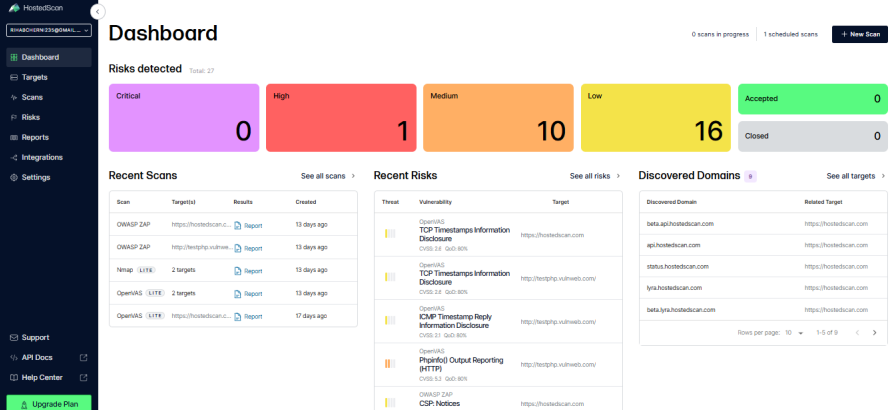
\includegraphics[width=\textwidth]{chapitres/ch1/img/existant/hostedscan.PNG}
                    \caption{Interface du l’application Hostedscan\cite{hostedscanimg}}
                    \label{fig:Hostedscan}
                \end{figure}
            \vspace{-0.1cm}
            \item \textbf{Invicti\cite{invicti} :} est un outil de sécurité web avancé permettant de protéger les applications, services web et API contre une large gamme de vulnérabilités, telles que les injections SQL, les failles \acs{XSS} et les erreurs de configuration SSL/TLS. Il réalise également des tests de configuration des serveurs web et se distingue par son moteur d’analyse basé sur la preuve, qui confirme automatiquement l’exploitabilité des failles détectées, réduisant ainsi les faux positifs. Son moteur d’exploration intelligent est compatible avec les technologies dynamiques modernes (JavaScript, Ajax, React, Angular), ce qui le rend efficace pour l’analyse des applications complexes.\\Invicti s’intègre facilement aux pipelines DevOps et CI/CD, favorisant une automatisation continue de la sécurité. Il propose en outre des tableaux de bord interactifs, des rapports personnalisables et des fonctionnalités de gestion des vulnérabilités, facilitant la collaboration entre les développeurs et les équipes de sécurité.
            
            La Figure~\ref{fig:Invicti} montre l’interface de l’outil Invicti, mettant en évidence les résultats d’analyse de sécurité web ainsi que les fonctionnalités de gestion des vulnérabilités.
            \begin{figure}[H]
                \centering
               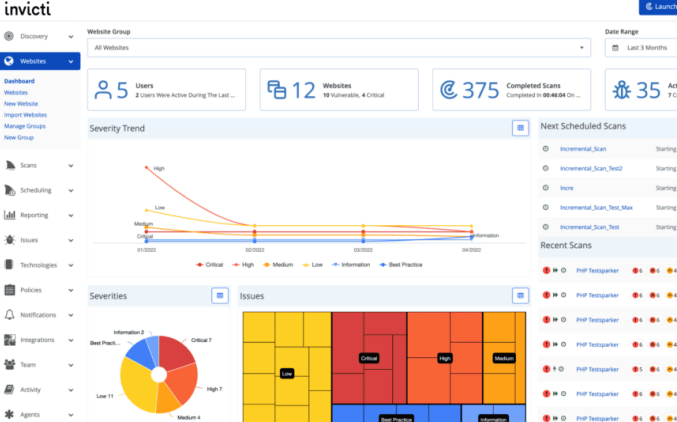
\includegraphics[width=\textwidth]{chapitres/ch1/img/existant/invicti.png}
                \caption{Interface du l’application Invicti\cite{invicti}}
                \label{fig:Invicti}
            \end{figure}
            \vspace*{-0.4cm}
        \end{enumerate}
    \subsubsection{Outils d’automatisation des tests fonctionnels:}
        L’automatisation des tests fonctionnels est essentiel pour assurer la qualité et la fiabilité des applications. Plusieurs outils sont disponibles qui offrent des fonctionnalités variées comme:
        \begin{enumerate}[label=\alph*)]
           \item  \textbf{Cypress}\cite{Cypress} est un outil d'automatisation de tests fonctionnels pour les applications web, apprécié pour sa rapidité, sa fiabilité et sa simplicité d'utilisation. Il permet d’automatiser des tests de composants, d’API et d’accessibilité, tout en assurant la compatibilité multi-navigateurs. Grâce à son interface de débogage en temps réel, son exécution locale rapide et sa facilité d’intégration, il constitue une solution complète pour les tests web.

           La Figure~\ref{fig:Cypress} illustre l’environnement de test automatisé proposé par Cypress, affichant les scénarios exécutés, les résultats des tests, et les options de débogage.
                \begin{figure}[H]
                \centering
               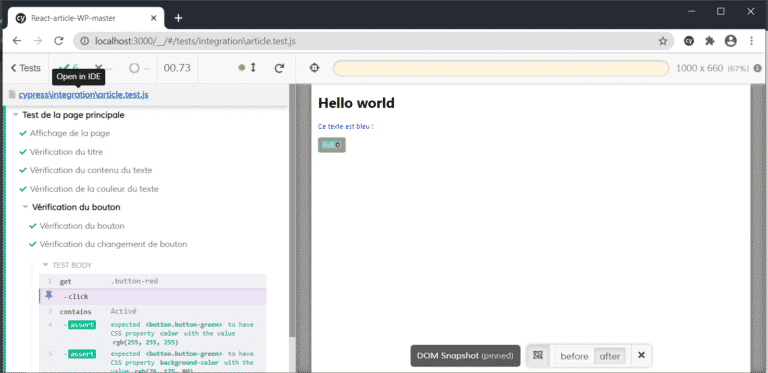
\includegraphics[width=\textwidth]{chapitres/ch1/img/existant/cpress.PNG}
               \caption{Interface de démonstration de Cypress exécutant une suite de tests \cite{imgCypress}}
                \label{fig:Cypress}
            \end{figure}
                \vspace{-0.4cm}
            \item  \textbf{Katalon Studio\cite{Katalon}:} est un outil d'automatisation des tests pour les applications web et mobiles, basé sur Selenium. Il offre une interface conviviale permettant de créer et d’exécuter des tests sans compétences techniques avancées. Son intégration avec des outils comme Jira et Slack, ainsi que son support des tests continus et du suivi instantané des résultats, en fait une solution efficace pour assurer la qualité tout au long du développement.

            La Figure~\ref{fig:Katalon-Studio} présente l’interface de Katalon Studio, illustrant l’organisation des cas de test ainsi que le suivi de leur exécution.
            \begin{figure}[H]
                \centering
                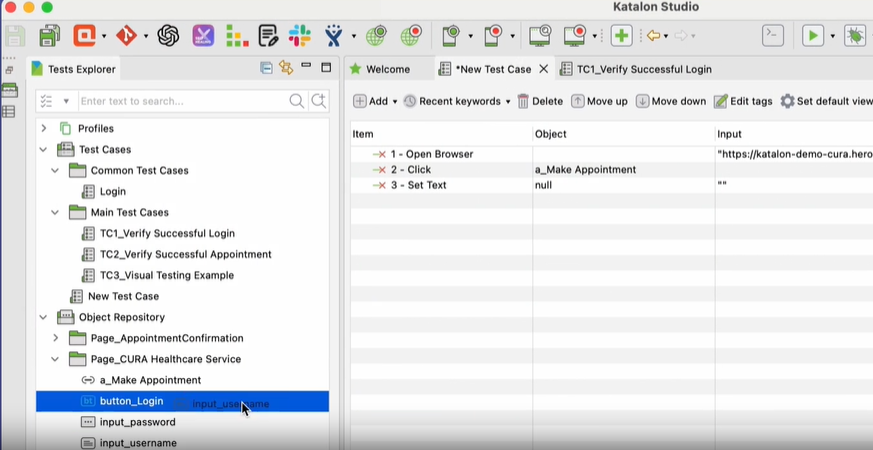
\includegraphics[width=\textwidth]{chapitres/ch1/img/existant/katal.PNG}
                \caption{Interface du l’application Katalon Studio\cite{Katalon}}
                \label{fig:Katalon-Studio}
            \end{figure}
            \vspace{-0.3cm}
    \end{enumerate}
    
    \subsubsection{Outils d’automatisation des tests SEO}
        Le \textbf{SEO (Search Engine Optimization)} est indispensable pour renforcer la visibilité d’un site sur les moteurs de recherche.Il permet d’identifier les erreurs, d’optimiser les performances et de vérifier le respect des bonnes pratiques. Plusieurs outils automatisent ces audits en analysant les mots-clés, le contenu, les aspects techniques, le positionnement, et en générant des recommandations et des rapports. Voici une analyse des plus pertinents.  
        \begin{enumerate}[label=\alph*)]
            \item \textbf{Semrush\cite{seoTools}:} est un outil SEO les plus populaires et complets du marché. Il propose une large gamme de fonctionnalités: l’analyse de mots-clés, l’audit technique, la veille concurrentielle, le suivi de positionnement, la gestion des backlinks, l’analyse du temps moyen passé sur le site ainsi que l’identification des pages les plus performantes. Son outil de suivi de positionnement fournit des analyses précises et évolutives, permettant aux professionnels du marketing digital de surveiller efficacement la performance de leurs mots-clés sur les moteurs de recherche. Il permet également de réaliser des audits SEO détaillés et de générer des rapports visuels pour le suivi des performances dans le temps.

            La Figure~\ref{fig:Semrush} illustre le tableau de bord de SEMrush, mettant en évidence les résultats de l’audit SEO ainsi que les performances globales du site web.
            \begin{figure}[H]
                \centering
                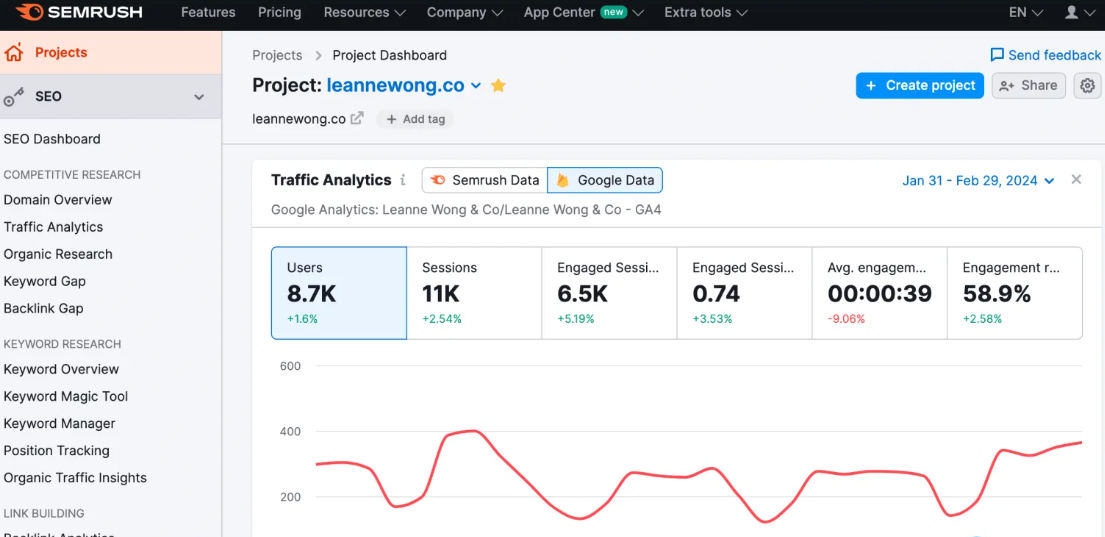
\includegraphics[width=\textwidth]{chapitres/ch1/img/existant/semrush.PNG}
                \caption{Interface de l’outil Semrush\cite{seoTools}}
                \label{fig:Semrush}
            \end{figure}
        \vspace{-0.3cm}
        \item \textbf{Ahrefs\cite{seoTools}} est une plateforme SEO reconnue pour la puissance de sa base de données de backlinks et ses capacités avancées d’analyse concurrentielle. Elle permet d’ajuster efficacement sa stratégie de contenu en observant les performances des concurrents sur les moteurs de recherche. L’outil offre des fonctionnalités telles que le suivi du positionnement des mots-clés, l’identification des pages les plus génératrices de trafic, l’analyse des liens entrants et l’accès à l’historique du positionnement via des visualisations graphiques.

        La Figure~\ref{fig:AhrefsAudit} présente l’interface d’Ahrefs, mettant en évidence le suivi du positionnement ainsi que les principaux indicateurs de performance SEO.
            \begin{figure}[H]
                \centering
                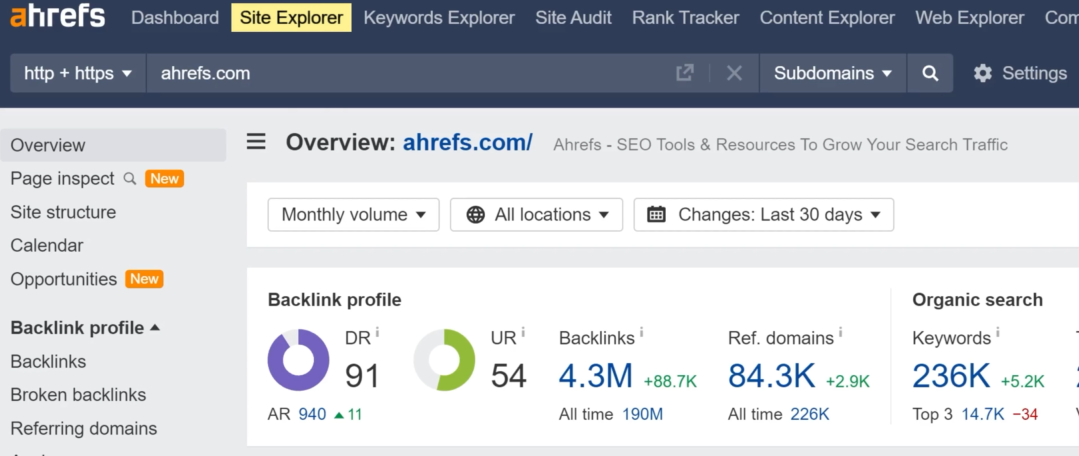
\includegraphics[width=\textwidth]{chapitres/ch1/img/existant/ahrefs.PNG}
                \caption{Interface de l’outil Ahrefs Site Audit\cite{seoTools}}
                \label{fig:AhrefsAudit}
            \end{figure}
            \vspace{-0.3cm}
        \end{enumerate}    
    \subsubsection{Critique de l’existant:}
        Le tableau ~\ref{tab: comparaison} présente une  comparaison détaillée des principaux outils analysés précédemment.
        \begin{spacing}{1.5}
            \begin{longtable}{|p{2.7cm}|p{6.6cm}|p{6.6cm}|}
                \caption{\centering Tableau comparatif des outils d’automatisation}
                \label{tab: comparaison}\\ \hline
                         \multicolumn{3}{|c|}{\textbf{Outils d’automatisation des tests de pénétration \cite{etdeExistant}}} \\
                        \hline
                        \textbf{Application} & \textbf{HostedScan} & \textbf{Invicti}\\
                        \hline
                            \textbf{Score}\footnote{Le score Geekflare est attribué par une équipe éditoriale selon plusieurs critères techniques et fonctionnels (source : \href{https://geekflare.com/fr/cybersecurity/best-website-security-scanner/}{Geekflare}).}& 
                                4.2/5 &
                                4.5/5
                                \\  \hline
                             \begin{minipage}[t]{2.8cm}
                                \textbf{Profondeur d’analyse}
                            \end{minipage}& 
                            \begin{minipage}[t]{6.6cm}
                                 \justifying Réseaux, serveurs, applications web
                            \end{minipage}
                                &
                             \begin{minipage}[t]{6.6cm}
                                 \justifying API, sites, applications, services et serveurs web.
                                 \vspace{0.2cm}
                            \end{minipage}
                            \\ 
                        \hline
                             \begin{minipage}[t]{2.9cm}
                                 \textbf{Fonctions principales}
                            \end{minipage}& 
                            \begin{minipage}[t]{6.6cm}
                                 \justifying Scanners open-source et gestion centralisée des vulnérabilités.
                            \end{minipage}
                                &
                            \begin{minipage}[t]{6.6cm}
                                 \justifying Analyse basée sur la preuve et exploitation automatique des vulnérabilités.
                                \vspace{0.2cm}
                            \end{minipage}\\ 
                        \hline
                            \textbf{Avantages} & 
                                \begin{minipage}[t]{6.6cm}
                                     \justifying
                                    \begin{itemize}[left=-0.1cm, label=\textcolor{green}{$\checkmark$}]
                                        \item Détection et notification en temps réel des menaces  
                                        \item Analyse approfondie.
                                        \item Rapports personnalisables.
                                        \item Offre un plan gratuit.  
                                    \end{itemize}
                                    \vspace{0.1cm}
                                \end{minipage}
                                &
                                \begin{minipage}[t]{6.6cm}
                                     \justifying 
                                    \begin{itemize}[left=-0.1cm, label=\textcolor{green}{$\checkmark$}]
                                        \item Excellent support client.
                                        \item Fournit des rapports et des analyses détaillés.
                                        \item Faible nombre de faux positifs.
                                    \end{itemize}
                                \end{minipage}\\ 
                            \hline
                            \textbf{Inconvénients} & 
                                \begin{minipage}[t]{6.6cm}
                                     \justifying
                                    \begin{itemize}[left=-0.1cm, label=\textcolor{red}{\ding{56}}]
                                        \item Interface utilisateur peu ergonomique  
                                         \item Limité aux scanners open-source 
                                    \end{itemize}
                                    \vspace{0.1cm}
                                \end{minipage} &
                                \begin{minipage}[t]{6.6cm}
                                     \justifying
                                    \begin{itemize}[left=-0.1cm, label=\textcolor{red}{\ding{56}}]
                                        \item Absence de tarification initiale.
                                        \item Les analyses prennent parfois beaucoup de temps
                                    \end{itemize}
                                \end{minipage}\\
                            \hline
                            \textbf{Tarification} & 
                               \begin{minipage}[t]{6.6cm}
                                     \justifying
                                    \begin{itemize}[left=-0.1cm, label=$\bullet$]
                                        \item \textbf{Gratuit}: 3 analyses par mois  
                                        \item \textbf{Basique}: 39\$ mois  
                                        \item \textbf{Premium}:109\$ mois
                                    \end{itemize}
                                    \vspace{0.1cm}
                                \end{minipage}
                                &
                                \begin{minipage}[t]{6.6cm}
                                     \justifying  Offre des prix personnalisés en fonction de vos besoins spécifiques.
                                \end{minipage}\\ 
                           \hline
    
                          \multicolumn{3}{|c|}{\textbf{Outils d’automatisation des tests fonctionnels\cite{,compTestFon2}}} \\
                        \hline
                        
                        \textbf{Application} & \textbf{Cypress} & \textbf{Katalon Studio} \\
                        \hline
                            \textbf{Score}\footnote{Le score Capterra reflète la moyenne des avis des utilisateurs sur différents critères (ergonomie, fonctionnalités, support, rapport qualité/prix)(source: \href{https://clickup.com/fr-FR/blog/228197/les-outils-de-test-d'automatisation}{ClickUp}).}
                            & 4.7/5& 4.4/5 \\ 
                        \hline
                            \begin{minipage}[t]{2.8cm}     
                                \textbf{Profondeur d’analyse}
                            \end{minipage}& 
                            \begin{minipage}[t]{6.6cm}
                                 \justifying Tests: de bout en bout, de composants, d’API, d'accessibilité.
                                 \vspace{0.1cm}
                            \end{minipage}
                                & 
                            \begin{minipage}[t]{6.6cm}
                                 \justifying Tests: UI, d'API, de charge, de performance des applications web.
                                \vspace{0.1cm}
                            \end{minipage} 
                            \\ 
                        \hline
                            \textbf{Avantages} & 
                                \begin{minipage}[t]{6.8cm}
                                    \begin{itemize}[left=-0.1cm, label=\textcolor{green}{$\checkmark$}]
                                        \item Exécution rapide, compatible multi-navigateurs.
                                        \item Facilité de configuration.
                                        \item Débogage puissant avec l'interface graphique.
                                        \item Tests fiables et résultats cohérents.
                                    \end{itemize}
                                    \vspace{0.1cm}
                                \end{minipage}
                                &
                                \begin{minipage}[t]{6.6cm}
                                     \justifying
                                    \begin{itemize}[left=-0.12cm, label=\textcolor{green}{$\checkmark$}]
                                        \item Facilité d'utilisation.
                                        \item Documentation complète et support client efficace.
                                        \item Intégration facile avec les pipelines CI/CD.
                                        \item Compatibilité multi-navigateurs et tests multiplateformes.
                                    \end{itemize}
                                    \vspace{0.1cm}
                                \end{minipage}
                                \\ 
                        \hline
                            \textbf{Inconvénients} & 
                                \begin{minipage}[t]{6.6cm}
                                     \justifying
                                    \begin{itemize}[left=-0.1cm, label=\textcolor{red}{\ding{56}}]
                                        \item Certains utilisateurs ont constaté des bugs.
                                        \item Manque d'assistance intégrée pour les tests d'applications mobiles.
                                    \end{itemize}
                                \end{minipage} &
                                \begin{minipage}[t]{6.6cm}
                                     
                                    \justifying
                                    \begin{itemize}[left=-0.1cm, label=\textcolor{red}{\ding{56}}]
                                        \item Décalage lors de l'utilisation sur certains ordinateurs portables.
                                        \item Des fonctionnalités manquantes comme l'exécution parallèle.
                                    \end{itemize}
                                    \vspace{0.1cm}
                                \end{minipage}  \\
                        \hline
                            \textbf{Tarification} & 
                               \begin{minipage}[t]{6.6cm}
                                    \begin{itemize}[left=-0.1cm, label=$\bullet$]
                                        \item \textbf{Gratuit}: Plan communautaire limité
                                        \item \textbf{Équipes}: 75\$/mois.
                                        \item \textbf{Business}: 300\$/mois
                                        \item \textbf{Entreprise}: Prix personnalisé.
                                    \end{itemize}
                                    \vspace{0.1cm}
                                \end{minipage}&
                                 \begin{minipage}[t]{6.6cm}
                                     \justifying
                                    \begin{itemize}[left=-0.15cm]
                                        \item[$\bullet$] \textbf{Gratuit}: 0\$ (Plan de base avec certaines limitations).
                                        \item[$\bullet$] \textbf{Premium}: 218\$/utilisateur/mois  
                                        \item[$\bullet$] \textbf{Entreprise}: Prix personnalisé.
                                    \end{itemize}
                                    \vspace{0.1cm}
                                \end{minipage} 
                                \\ 
                       \hline
                       \multicolumn{3}{|c|}{\textbf{Outils d’audit SEO automatisé\cite{seoTools}}} \\
                        \hline
                        \textbf{Application} & \textbf{Semrush}& \textbf{Ahrefs Site Audit} \\
                        \hline
                            \textbf{Score}\footnote{Le score Capterra correspond à la moyenne des avis utilisateurs, évaluant des critères tels que l’ergonomie, les fonctionnalités, le support et le rapport qualité/prix (sources : \href{https://www.capterra.com/p/176340/Ahrefs/}{Ahrefs} et \href{https://www.capterra.com/p/151962/SEMrush/}{SEMrush}).}
                            & 4.6/5& 4.7/5 \\ 
                        \hline 
                        \textbf{Interface utilisateur} & 
                        Simple, intuitive et rapide à utiliser & 
                        Tableaux de bord graphiques et interactifs \\
                        \hline   
                        \textbf{Fonctions principales} & 
                        Audit HTML, SEO on-page, détection de liens cassés, analyse de la vitesse, compatibilité mobile, avec export des 1résultats en PDF & Visualisation graphique, suivi des erreurs, historique des audits, recommandations, avec export des résultats sous forme de graphiques et de rapports web \\
                        \hline
                        \textbf{Avantages} & 
                       \begin{minipage}[t]{6.6cm}
                            \begin{itemize}[left=-0.15cm, label=\textcolor{green}{$\checkmark$}]
                               \item Recherche et suivi des mots-clés.
                               \item Analyse concurrentielle.
                               \item Suivi du positionnement en temps réel.
                               \item Audit technique SEO complet.
                               \item Optimisation des backlinks.
                               \item Interface personnalisable.
                             \end{itemize}
                        \end{minipage}& 
                         \begin{minipage}[t]{6.6cm}
                            \begin{itemize}[left=-0.15cm, label=\textcolor{green}{$\checkmark$}]
                                \item Base de données de backlinks ultra-complète.
                                \item Analyse approfondie des sites concurrents pour identifier leurs stratégies SEO.
                                \item Suivi précis des performances et suggestions de contenu pertinentes.
                            \end{itemize} 
                            \vspace{0.05cm}
                        \end{minipage}\\
                        \hline 
                        \textbf{Inconvénients} & 
                         \begin{minipage}[t]{6.6cm}
                            \begin{itemize}[left=-0.15cm, label=\textcolor{red}{\ding{56}}]
                                \item Tarification élevée pour les petites entreprises.
                                \item Une interface complexe pour les débutants.
                            \end{itemize}
                            \vspace{0.1cm}
                        \end{minipage}& 
                         \begin{minipage}[t]{6.6cm}
                            \begin{itemize}[left=-0.15cm, label=\textcolor{red}{\ding{56}}]
                                \item Moins complet que Semrush pour l’optimisation on-site.
                                \item Peu d’options pour générer des rapports personnalisés.
                            \end{itemize}
                            \vspace{0.1cm}
                        \end{minipage}\\
                        \hline
                    \end{longtable}
        \end{spacing}
        \vspace{-0.4cm}
        Chaque outil présente des atouts spécifiques selon le type de tests à automatiser, qu’il s’agisse de sécurité, de fonctionnalité ou d’audit SEO. Le choix de l’outil dépendra des besoins techniques, du budget disponible et du niveau d’intégration souhaité dans le processus de développement.
\end{justify}
    \section{Problématique}
        Les tests fonctionnels, les tests de sécurité ainsi que les tests SEO représentent trois aspects essentiels pour garantir la fiabilité, la performance et la visibilité des applications. Toutefois, leur mise en œuvre reste principalement manuelle, ce qui la rend chronophage et sujette à des erreurs humaines. \\
La question qui se pose est de concevoir une solution capable d’automatiser ces types de tests tout en assurant une couverture complète et une analyse fiable?



    \section{Solution proposée}
        Afin de surmonter les nombreuses limites identifiées dans l’application existante, la solution proposée vise à développer une plateforme complète pour l’automatisation des tests de sécurité, des audits SEO, et des tests fonctionnels avec une analyse fiable et complète des résultats. Elle vise à renforcer la visibilité des applications tout en garantissant leur bon fonctionnement. Cette nouvelle solution repose sur une approche intégrée et évolutive avec les objectifs suivants:
\begin{itemize}[label=$\bullet$,left=0.09cm]
    \item \textbf{Intégration optimisée des outils de pénétration}: Utilisation de ZAP\cite{zap}, Wapiti\cite{wapiti}, Nuclei\cite{nuclei}, Nikto\cite{nikto}, SQLMap\cite{sqlmap}, XSStrike\cite{xsstrike} et autres, chacun spécialisé dans une famille de vulnérabilités, pour détecter les failles de sécurité et couvrir un périmètre d’analyse plus large et plus fiable.
    
    \item \textbf{Mécanisme de comparaison, de consolidation des résultats et de validation automatique des faux positifs}: regroupement des vulnérabilités similaires détectées par différents outils, avec une pondération selon leur niveau de risque, afin d’éliminer les doublons, de clarifier les rapports, d’améliorer leur précision, de filtrer les résultats pertinents, de réduire les erreurs de détection et d’optimiser le temps d’analyse.

    \item \textbf{Scan d’authentification automatisé}: Détection des formulaires de connexion après identification des champs login/password, cookies et tokens d’authentification pour permettre les scans dans les zones protégées en reproduisant des scénarios d’attaque.
    
    \item \textbf{Automatisation des tests fonctionnels}: en exécutant des scénarios de tests simulant le comportement utilisateur (remplissage de formulaires, clics, redirections), afin de vérifier que les fonctionnalités clés restent opérationnelles et conformes aux exigences des utilisateurs.
    
    \item \textbf{Automatisation des tests SEO}: pour analyser les techniques du référencement (temps de chargement, structure HTML, balises, liens cassés).
    
    \item \textbf{Système de reporting}: Génération de rapports synthétiques et clairs avec des filtres (par outil, par niveau de gravité, par catégorie), visualisation graphique interactive, export en PDF, HTML, JSON ou CSV, envoi par e-mail, Slack ou Jira.
    \item \textbf{Refonte de la base de données} : adoption d’une structure relationnelle optimisée avec des tables normalisées permettant un stockage détaillé des rapports, une gestion granulaire des vulnérabilités ainsi qu’une meilleure exploitation des données via des requêtes avancées.
    \item \textbf{Gestion intelligente des scans concurrents} : Mise en place d’un système de file d’attente et de verrouillage par utilisateur afin d’empêcher le lancement simultané ou successif non contrôlé de plusieurs scans. Une logique de planification permet d’exécuter les scans de manière ordonnée, tout en assurant un contrôle d’accès aux ressources partagées. Des vérifications en temps réel préviennent les doublons, les surcharges ou les blocages. Des statuts d’exécution offrent à l’utilisateur la possibilité de suivre l’avancement d’un scan ou de l’annuler si nécessaire.
    \item \textbf{Interface responsive et modernisée}: Refonte complète du frontend en Angular dernière version 18, accès contrôlé par authentification JWT\cite{jwt} et rôle utilisateur, et responsive design pour mobile et tablette.
    \item \textbf{Sécurisation complète des accès} : Mise en place d’un contrôle d’accès uniforme sur l’ensemble des routes, avec redirections automatiques, gestion des sessions et mécanisme de réinitialisation de mot de passe.
\end{itemize}
Cette solution permettra de corriger en profondeur les failles de l’application actuelle en rendant les processus de tests efficaces et compréhensibles. Elle contribuera aussi à fournir une plateforme unifiée adaptée aux besoins réels des développeurs, des testeurs et des responsables sécurité.

    \section{Choix méthodologique de travail}
    Les méthodes agiles proposent une approche flexible et itérative du développement, centrée sur la réduction des risques, l’adaptabilité et la satisfaction du client. Scrum est la méthode agile la plus couramment adoptée\cite{agile}.

Le choix méthodologique retenu pour notre application, défini dès le début du stage, résulte d’une réflexion collective. Il a été guidé par les besoins du projet et la stratégie de l’entreprise, notamment en matière d’approche, de langage de modélisation et de processus de développement.
\subsection{Fonctionnement général de Scrum\cite{Scrum}}
Scrum repose sur des itérations successives "sprints", comme l’illustre la figure \ref{fig:Scrum}, permettant une livraison progressive du produit et visant à apporter de la valeur au client en favorisant la transparence, la collaboration et l’amélioration continue.
\begin{figure}[H]
    \centering
    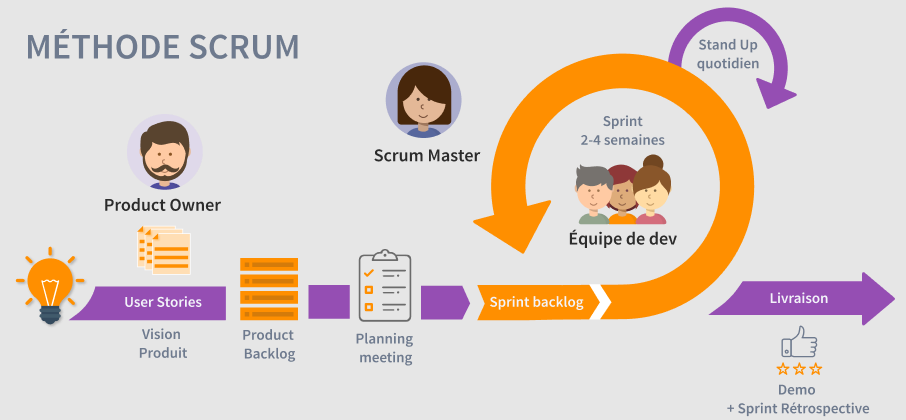
\includegraphics[width=\linewidth]{chapitres/ch1/img/scrum.PNG}
    \caption{Cadre méthodologique et mode de fonctionnement SCRUM \cite{ScrumImg}}
    \label{fig:Scrum}
\end{figure}
\vspace{-0.5cm}
L’équipe Scrum se compose de trois rôles clés:
\begin{itemize}[label=$\bullet$]
    \item \textbf{Product Owner:} Gère le backlog et définit les priorités selon les besoins client.
    \item \textbf{Scrum Master:} Garantit le respect de la méthodologie et facilite le travail de l’équipe.
    \item \textbf{Équipe de développement:} Chargée de la réalisation des fonctionnalités et de la livraison des incréments du produit.
\end{itemize}
\subsection{Événements Scrum\cite{Scrum}}
    Les événements Scrum assurent l’organisation et l’amélioration continue du processus:
    \begin{itemize}[label=$\bullet$]
        \item \textbf{Daily Scrum:} Réunion quotidienne de 15 minutes pour synchroniser le travail, partager les avancées et identifier les obstacles.
        \item \textbf{Sprint Review:} Présentation de l’incrément réalisé à la fin du sprint aux parties prenantes afin d'obtenir des retours et ajuster les priorités.
        \item \textbf{Sprint Retrospective:} Réunion d’équipe pour analyser ce qui a bien fonctionné, identifier les axes d’amélioration et optimiser les processus pour les futurs sprints.
    \end{itemize}
\subsection{Artefacts Scrum\cite{Scrum}}
    Les artefacts Scrum structurent le travail et assurent la transparence pour suivre l'évolution du projet et adapter les actions en conséquence. Parmi ces artefacts, on trouve :
    \begin{itemize}[label=$\bullet$]
        \item \textbf{Backlog produit :} liste évolutive des fonctionnalités, gérée par le \textbf{Product Owner}.
        \item \textbf{Backlog de sprint :} ensemble des tâches à réaliser durant un sprint.
        \item \textbf{Incrément de produit :} version fonctionnelle et enrichie du produit, livrée à la fin du sprint.
        \item \textbf{Burndown chart :} graphique illustrant l'avancement des tâches et la vélocité de l’équipe.
    \end{itemize}
\subsection{Avantages de Scrum\cite{Scrum}}
L’adoption de Scrum présente plusieurs avantages :
\begin{itemize}[label=$\bullet$]
    \item Meilleure qualité logicielle grâce aux tests fréquents et aux retours d’utilisateurs.
    \item Satisfaction client accrue, avec une réactivité face aux évolutions des besoins.
    \item Livraisons plus rapides, optimisant la mise en production des fonctionnalités prioritaires.
    \item Dynamique d’équipe améliorée, favorisant la motivation et l’autonomie des développeurs.
\end{itemize}  
    \section*{\texorpdfstring{Conclusion}{Conclusion}}
    \addcontentsline{toc}{chapter}{\textbf{Conclusion}}
    Ce chapitre a introduit le projet en présentant son contexte, les caractéristiques de l’organisme d’accueil, ainsi que les lacunes de l’outil existant et des solutions similaires, soulignant ainsi la nécessité d’adopter une nouvelle approche. Il a exposé la solution proposée et la méthodologie de travail. Le chapitre suivant portera sur l’analyse préliminaire de cette nouvelle solution.
\end{justify}